\chapter{Recommender System} \label{chap:Recommender}

\section{Choosing A Recommender Algorithms} \label{chooseRecAlg}
There are multiple different ways of implementing recommender system. For a machine learning approach there, there are three popular approaches used which are
\begin{itemize}
    \item Content-based filtering
    \item Collabortive filtering
    \item Hybrid Technique
\end{itemize}
as shown in figure \ref{fig:recommenderSystemTypes}. The main feature that the approaches listed above is similarity.

\begin{figure}[ht]
    \centering
    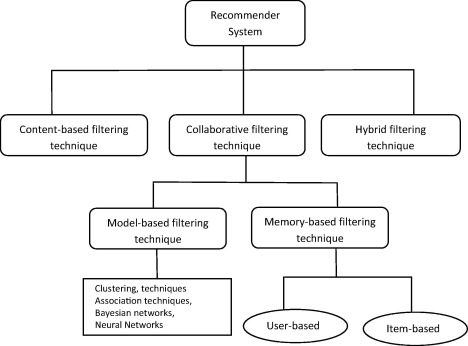
\includegraphics[width=\textwidth]{recommenderSystemTypes.jpg}
    \caption{Types of Recommender Systems}
    \label{fig:recommenderSystemTypes}
\end{figure}

\subsubsection{Content-based filtering}
With content-based filtering, you have meta-data about the particular items. So in our scenario we would have extra information about routes such as the type of terrain, location, elevation, etc. When a user runs a specific route, we suggest routes that are similar based on the extra meta-data provided

The main problem with this approach is providing the extra meta-data on the routes. We can get some of this data automatically by e.g. Calculating elevation as shown in section \ref{elevationProfile}, however, other information like the type of terrain cannot be achieved automatically. Another way is to get user's to add the extra information on the trails, but the system would then have to trust the user's knowledge on information of trails. The system would also then require a wide variety of attributes to categorise trails as there are multiple defining features for trails. Example shown in figure \ref{fig:contentBasedFiltering}
\begin{figure}[ht]
    \centering
    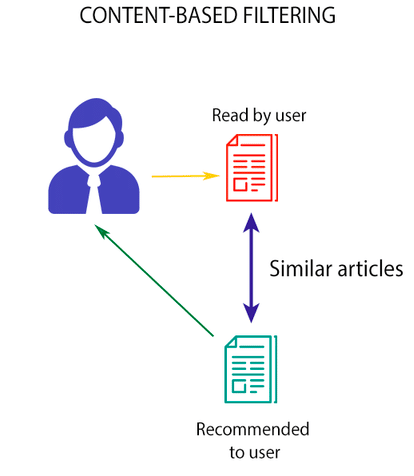
\includegraphics[width=0.5\textwidth]{content-based-filtering.png}
    \caption{Content based filtering}
    \label{fig:contentBasedFiltering}
\end{figure}

\subsubsection{Collaborative filtering}
Unlike content based filtering, collaborative filtering works on the similarity between users. The idea is that, user A likes routes 1 \& 2 and user B likes routes 2 \& 3. As user A and user B like the same route (route 2), then they are similar and user A would also like route 3. 

This property can be seen in real life and works extremely well. People are more likely to trust the suggestions of their friends, i.e. people that they are the most similar with. With this system, you do not need to know any extra information on the routes you are running the algorithm on. We us either explicit information such as user ratings, or implicit information such as number of views on a route, to determine the routes users like. Example shown in figure \ref{fig:collaborativeFiltering}.

Because of these reasons, I chose to use this type of recommender system.

\begin{figure}[ht]
    \centering
    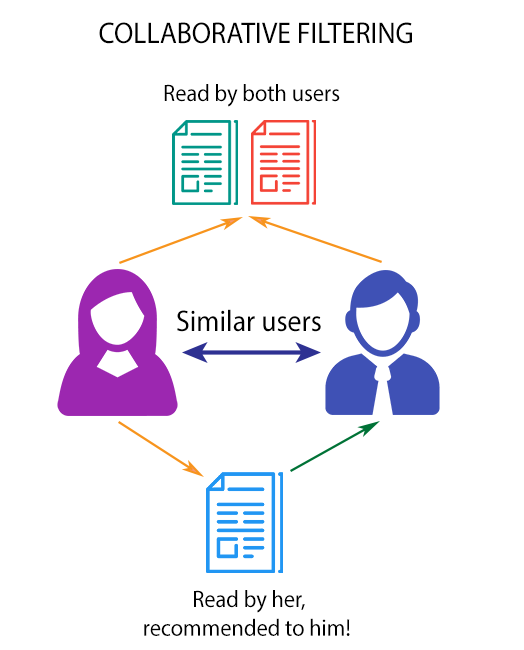
\includegraphics[width=0.5\textwidth]{collaborative-filtering.png}
    \caption{Collaborative filtering}
    \label{fig:collaborativeFiltering}
\end{figure}

\subsubsection{Hybrid Recommender Systems}
Hybrid recommender systems simply combine the results of both collaborative and content-based techniques. The results from both the system's would then have to be ranked again in the combiner as shown in figure \ref{fig:hybridRecommenderSystems}

\begin{figure}[ht]
    \centering
    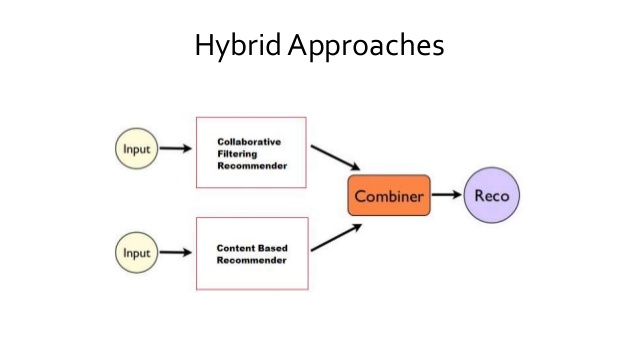
\includegraphics[width=0.5\textwidth]{hybrid-approaches.jpg}
    \caption{Hybrid Approaches}
    \label{fig:hybridRecommenderSystems}
\end{figure}


\section{Collaborative Filtering}
Collaborative filtering is based on the similarity score we can calculate using the explicit data we get from the users. The explicit data that we collect is a rating between 1-5\footnote{where 1 is the worst and 5 is the best}. We can either use a Memory based Technique or Model Based Technique.

\subsubsection{Memory based Technique}
With memory based techniques, we calculate similarity scores either between users or between items based on the ratings \cite{wang2006unifying}. 

The problem with this method is that it has to be run every time the user queries the system. Since there is no model to train as with most machine learning methods, you will have to calculate the similarity score with all the items each time which is a huge performance bottle neck.
\begin{figure}[ht]
    \centering
    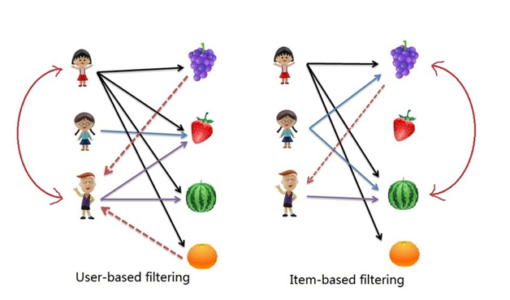
\includegraphics[width=\textwidth]{collab-filtering-types.png}
    \caption{Types of Collaborative filtering}
    \label{fig:collabFilteringTypes}
\end{figure}

\subsubsection{Model based techniques}
To improve on the issues of the memory based techniques, we can use model based techniques. We create a machine learning model that will be trained on a dataset of user-routes ratings using the Matrix Factorization method described in section \ref{matrixFactorization}. We will use a neural network described in section \ref{neuralNetwork}
\section{Matrix Factorization} \label{matrixFactorization}
For our Machine learning model we want to learn two features. 
\begin{itemize}
    \item what properties a specific user likes in routes
    \item what properties a route has that a route has
\end{itemize}
We can learn these features using a method called Matrix Factorization, which is one of the top methods proposed during the Netflix Prize \cite{bell2007lessons}.

Matrix Factorization is the process of decomposing a user-route rating matrix into a product of 2 lower dimensionality rectangular matrices \cite{koren2009bellkor} as shown in figure \ref{fig:matrixFactorization}.

\begin{figure}[ht]
    \centering
    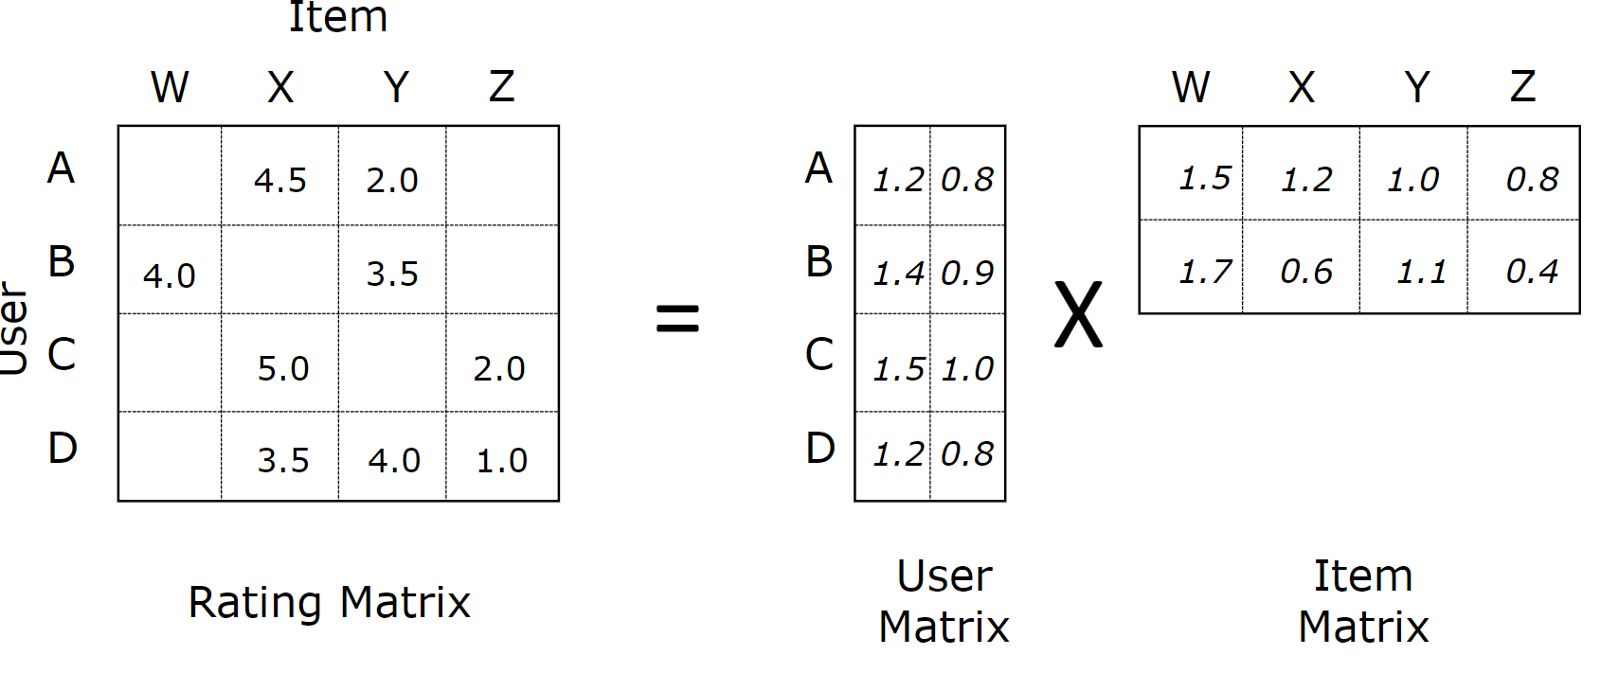
\includegraphics[width=\textwidth]{matrix-factorization.png}
    \caption{Example of Matrix Factorization}
    \label{fig:matrixFactorization}
\end{figure}

We can represent the above mathematically as
\begin{equation}
    R \approx P \times Q^T
\end{equation}

Given the type of rating matrix shown in figure \ref{matrixFactorization}, we want to predict what a user will rate the other items that they have not rate yet. This will allow us to predict what item's a user likes and suggest it to the user. What we try to do with Matrix factorization is learn the reason why users have rated the items that they have rated (assuming a user only rates items they use). These reasons are called Latent features\footnote{Latent is a synonym of Hidden}.

These features are latent because we do not initially know them, we don't even know if they exist. Our decomposed features are initialized to random values, and then we use a method called Gradient Decent to try and find what those values should be.

\subsection{Gradient Descent}
With our decomposed feature matrices, we want to optimize those values such that the product will be very similar to the original ratings matrix. We can do this using an optimization algorithm called Gradient Descent \cite{ruder2016overview}



\subsubsection{Loss Function}
With our training set, we know what the values of certain user-route ratings should be. When the predict the values of a features for these known values, we can calculate a predicted value for the user-route rating\footnote{using \url{http://www.quuxlabs.com/blog/2010/09/matrix-factorization-a-simple-tutorial-and-implementation-in-python/} for help here}

\begin{equation}
    \hat{r}_{ij} = {p^{T}_{j}}{q_j}=\sum_{k=1}^{k}{p_{ik}q_{ik}}
\end{equation}

With this predicted value, we can then calculate what is called our loss value. That is how wrong we are from the actual predicted value, we can calculate our loss value using the Mean Squared Error (MSE) Loss Function as shown in equation \ref{eqn:mseLossFunction}

\begin{equation} \label{eqn:mseLossFunction}
    MSE = \frac{1}{N}\sum_{i=1}^{N}{({f_i}-{y_i})}^2 
\end{equation}

What our gradient descent optimization function does is to try and minimize this values. By taking learning steps towards a minimum value similar to the image shown in figure \ref{fig:gradientDescent}. With gradient descent we back propagate these changes that are representatives as derivatives and change our initial feature matrix values and then run the method again, trying to further optimize our values. The gradient descent function that we use is call Adam \cite{kingma2014adam}.

\begin{figure}[ht]
    \centering
    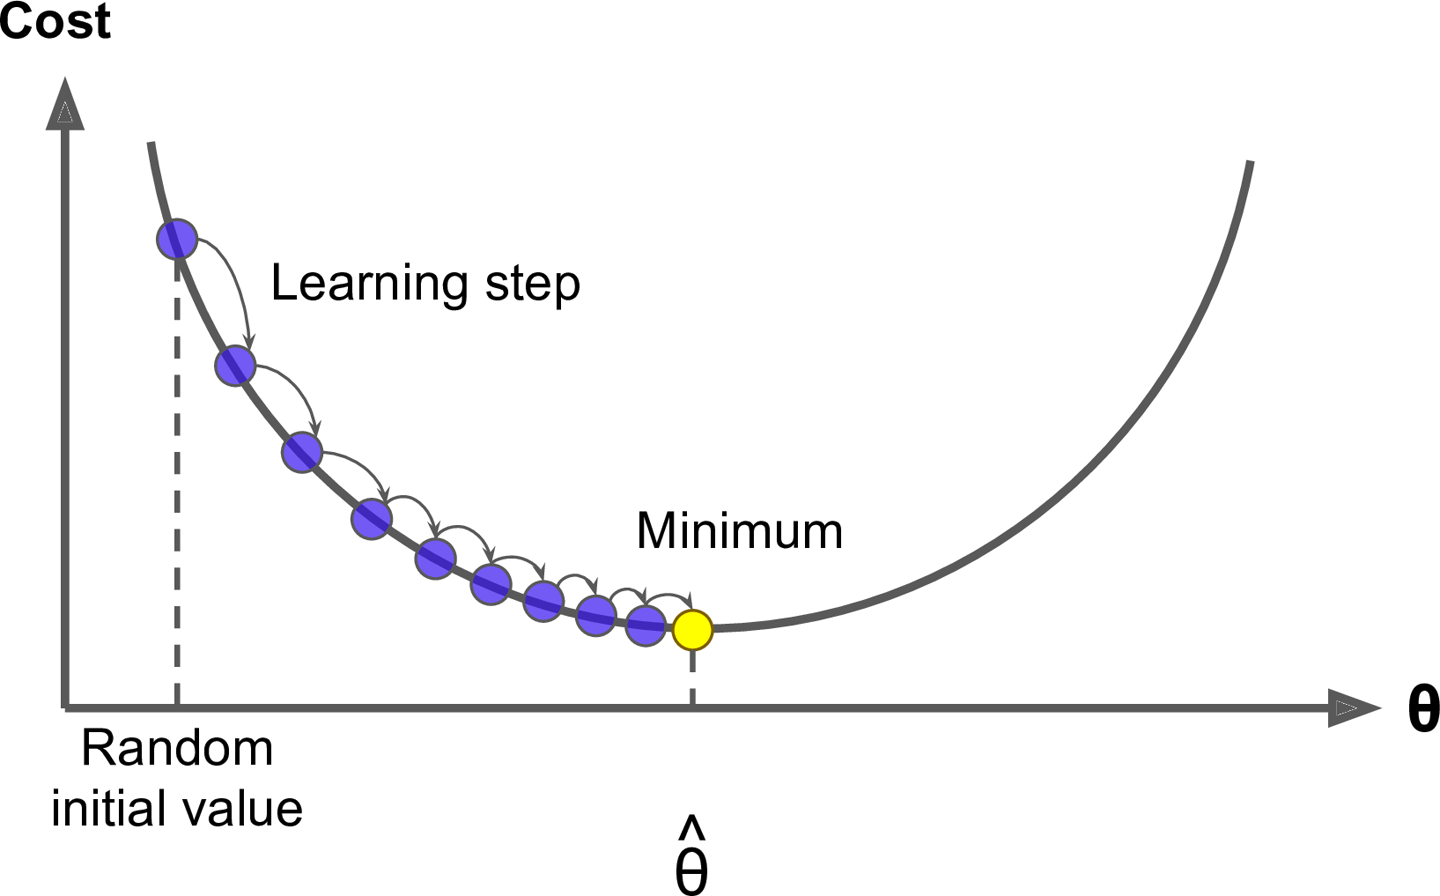
\includegraphics[width=\textwidth]{gradient-descent.png}
    \caption{Gradient Descent}
    \label{fig:gradientDescent}
\end{figure}

\subsection{Bias is a virtue}
To improve our model, we can introduce bias. In real life, you would trust a user that has run more routes than a user that has run fewer routes. This also applies for routes that have been run by more users. We can include this feature into our model to help improve the model created by adding bias values related to each user and each item (route). We include this bias in when training our model.

\begin{equation}
    \hat{r_{ui}} = \mu + b_i + b_u + {q^{T}_{i}}{p_u}
\end{equation}

\section{A Deep Learning Approach} \label{neuralNetwork}
Neural networks are modelled after the brains biological networks \cite{van2018artificial}. We can create our model discussed in section \ref{matrixFactorization}, using a neural network which is generally more Robust. Our neural network will use the initial feature matrices as our input to the neural networks. The hidden layer will consist of one dense layer with a ReLU activation function \cite{li2017convergence}, and then have a final output layer with one node. We use the same MSE as discussed before and use back-propagation to update our weights.

With the neural network, we can also add bias to help improve the model.

\begin{figure}[ht]
    \centering
    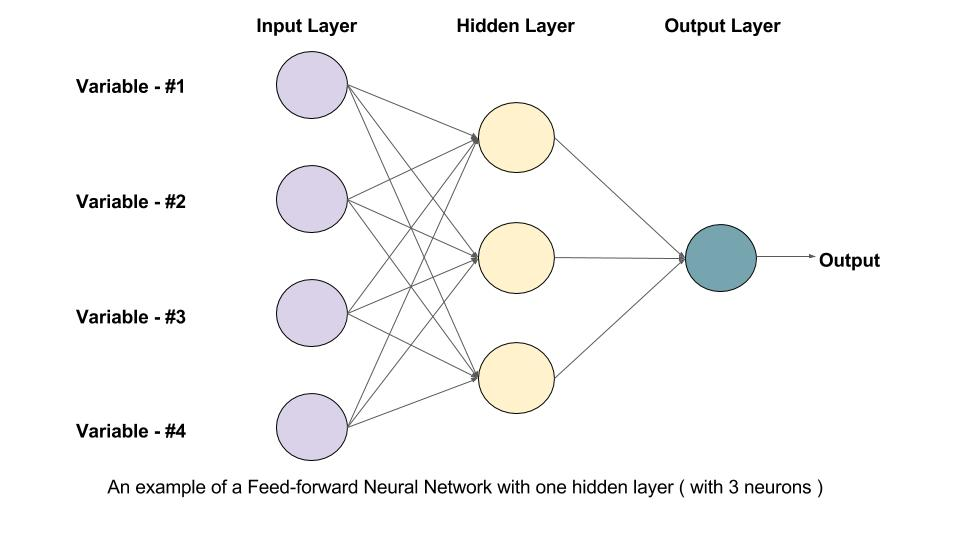
\includegraphics[width=\textwidth]{neural-net-example.jpg}
    \caption{Neural Network Example}
    \label{fig:neuralNetworkExample}
\end{figure}

\subsection{Preventing overfitting}
One of the main problems with machine learning approaches is over-fitting and under fitting.

\paragraph{Overfitting} is when our model is trained to match to perfectly with our training dataset and therefore has a hard time to predict when we have a completely new data. To prevent this in Neural Networks. Drop out layers kill random nodes in our neural network during each epoch. This forces the neural network to always try and learn new paths to during training preventing it form relying on the same weights each time.

\begin{figure}[ht]
    \centering
    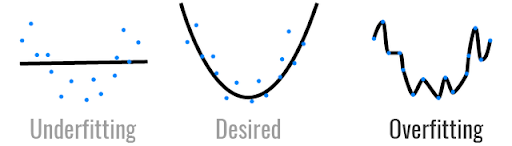
\includegraphics[width=\textwidth]{fitting-problem.png}
    \caption{Fitting Problems}
    \label{fig:fittingProblems}
\end{figure}


\begin{figure}[ht]
    \centering
    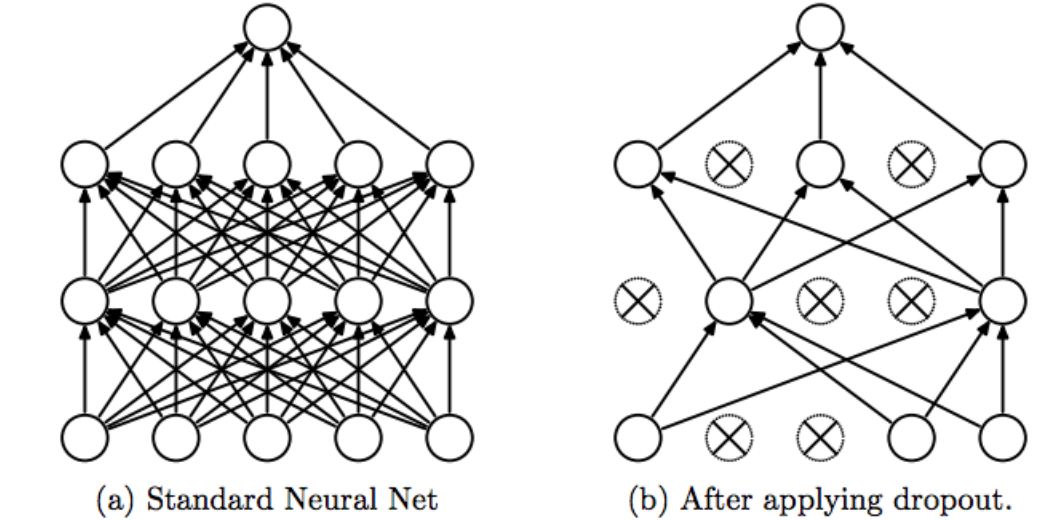
\includegraphics[width=\textwidth]{dropout.png}
    \caption{Dropout Layer}
    \label{fig:dropoutLayer}
\end{figure}
\section{Tensorflow and Python}
There are a few machine learning platforms that can help us to create our neural network. I decided to use tensorflow because it is popular and has a big community to help. It also is built with keras which allows you to create these models from a High Level. Tensor flow also has C++ bindings that takes use of the GPU for the matrix which is far more efficient than using a normal CPU and so is quicker for handling large datasets.

Tensorflow is mainly meant to be used in python as pytbon is the main language for Data Science. This proved to be a problem initially as I did not know python. Although Tensorflow also provides a javascript library\footnote{https://www.tensorflow.org/js}, I chose to use the python version as the javascript library did not provide all the functionality of the main python library. It also allowed me to use Jupyter Notebook (discussed in section \ref{jupyterNotebook}) which provided a really platform to experiment with the machine learning model.

\begin{figure}[ht]
    \centering
    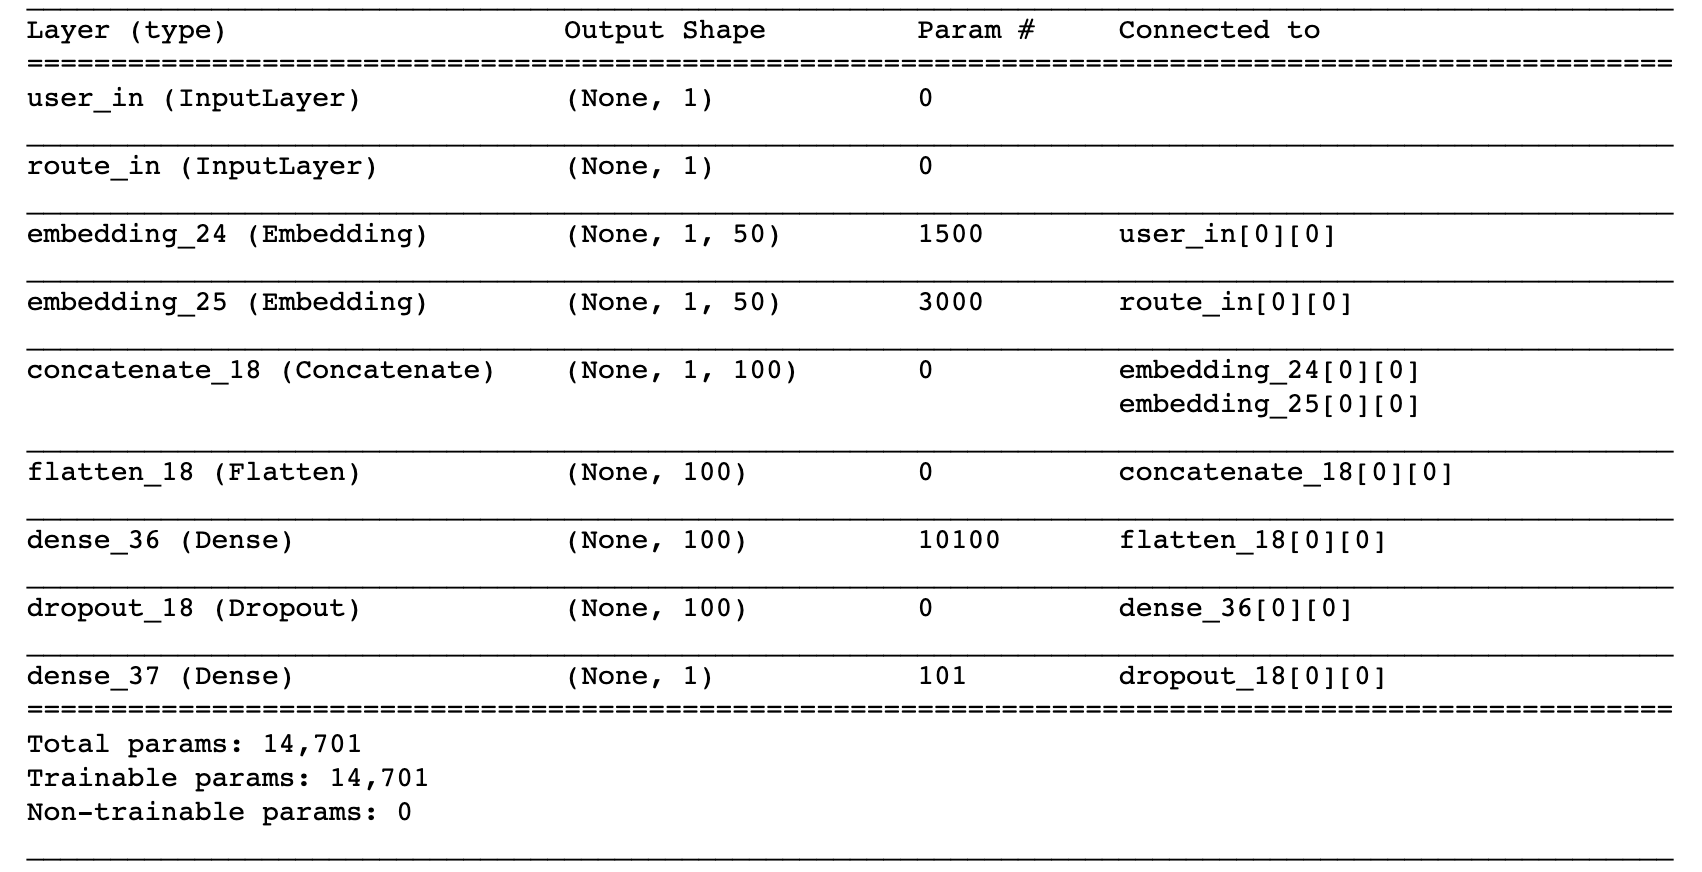
\includegraphics[width=\textwidth]{neural-net-summary.png}
    \caption{Summary of Neural Network}
    \label{fig:neuralNetworkSummary}
\end{figure}

\subsection{Jupyter Notebook} \label{jupyterNotebook}
Jupyter Notebook\footnote{https://jupyter.org/} that allows creating and running notebooks via a web appplication. These documents can contain both Markup text and more importantly code that is exists in cells on the document. The document allows you to easily share any code with others easily as it make's it straightforward to document. With it's use of cells, you can rerun individual blocks of code with running the entire document, making it easy to develop and iterate through different versions as you improve.
\begin{figure}[ht]
    \centering
    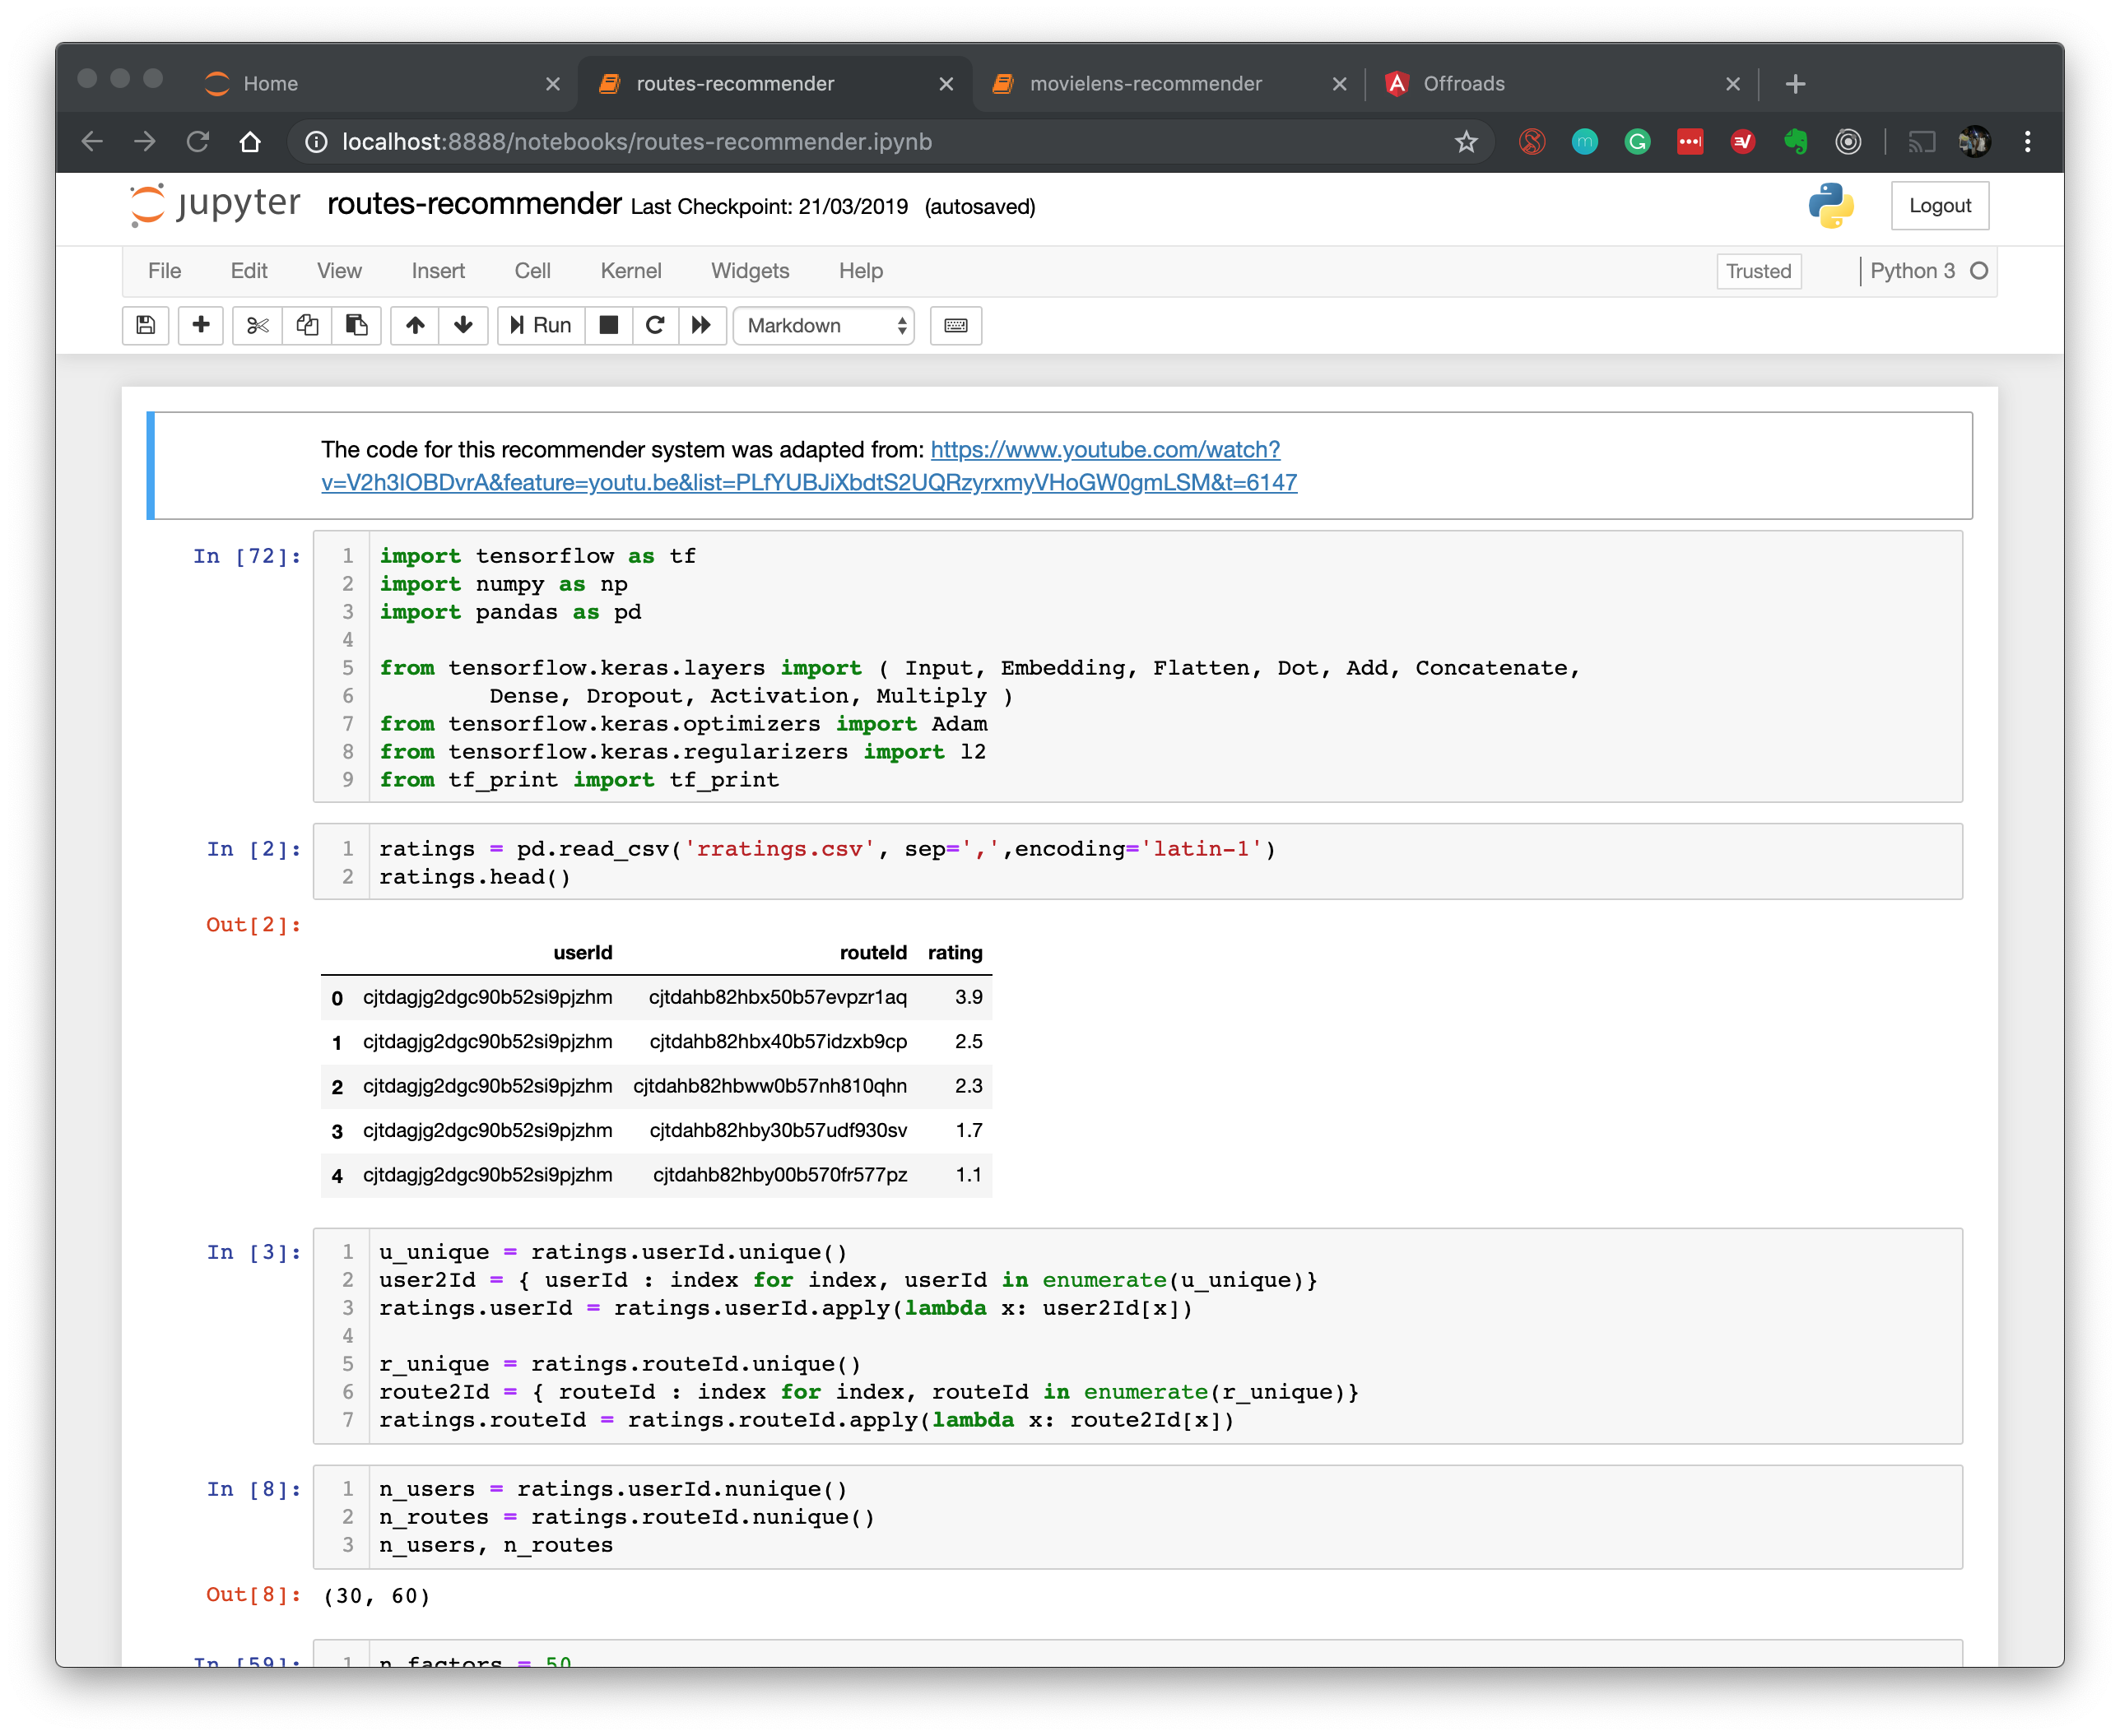
\includegraphics[width=\textwidth]{jupyter-notebook.png}
    \caption{Jupyter Notebook}
    \label{fig:JupyterNotebook}
\end{figure}

